

%% Lee
%% In dissertation, change section* to chapter and subsection* to section


\chapter{System Overview}
\label{chap-five}
\label{sec:System Overview}
As mentioned in chapter \ref{sec:Introduction} and chapter \ref{Motivation}, this works target application implements mulltiple \acp{ann} each of which have limited opportunities for both weight reuse and batch processing.
These requirements require \ac{dram} to be employed for main storage of \ac{ann} parameters and local \ac{sram} is of limited use.
Under these conditions, the \ac{dram} bandwidth is the system bottleneck.

To meet these requirements, this work proposed employing \acp{3dic} technology along with a customized \ac{3d} \ac{dram} and \ac{asic} technology. 
By physically staying within the \ac{3dic} footprint and taking advantage of high density \acp{tsv} this work is able to maintain a significantly higher bandwidth over 2D or 2.5D \ac{asic} or \ac{asip} solutions.
The objective was to demonstrate that a pure \ac{3dic} system can implement multiple disparate \acp{ann} within reasonable power and area constraints. 

The \ac{3dic} system die stack (figure \ref{fig:3DICStack}) includes the \ac{3d}-\ac{dram} with a system manager below and one or more processing layers below the manager.
\begin{figure}[!t]
% the [] contains position info e.g. [!t] means here
\centering
\captionsetup{justification=centering}
\captionsetup{width=.9\linewidth}
\centerline{
\mbox{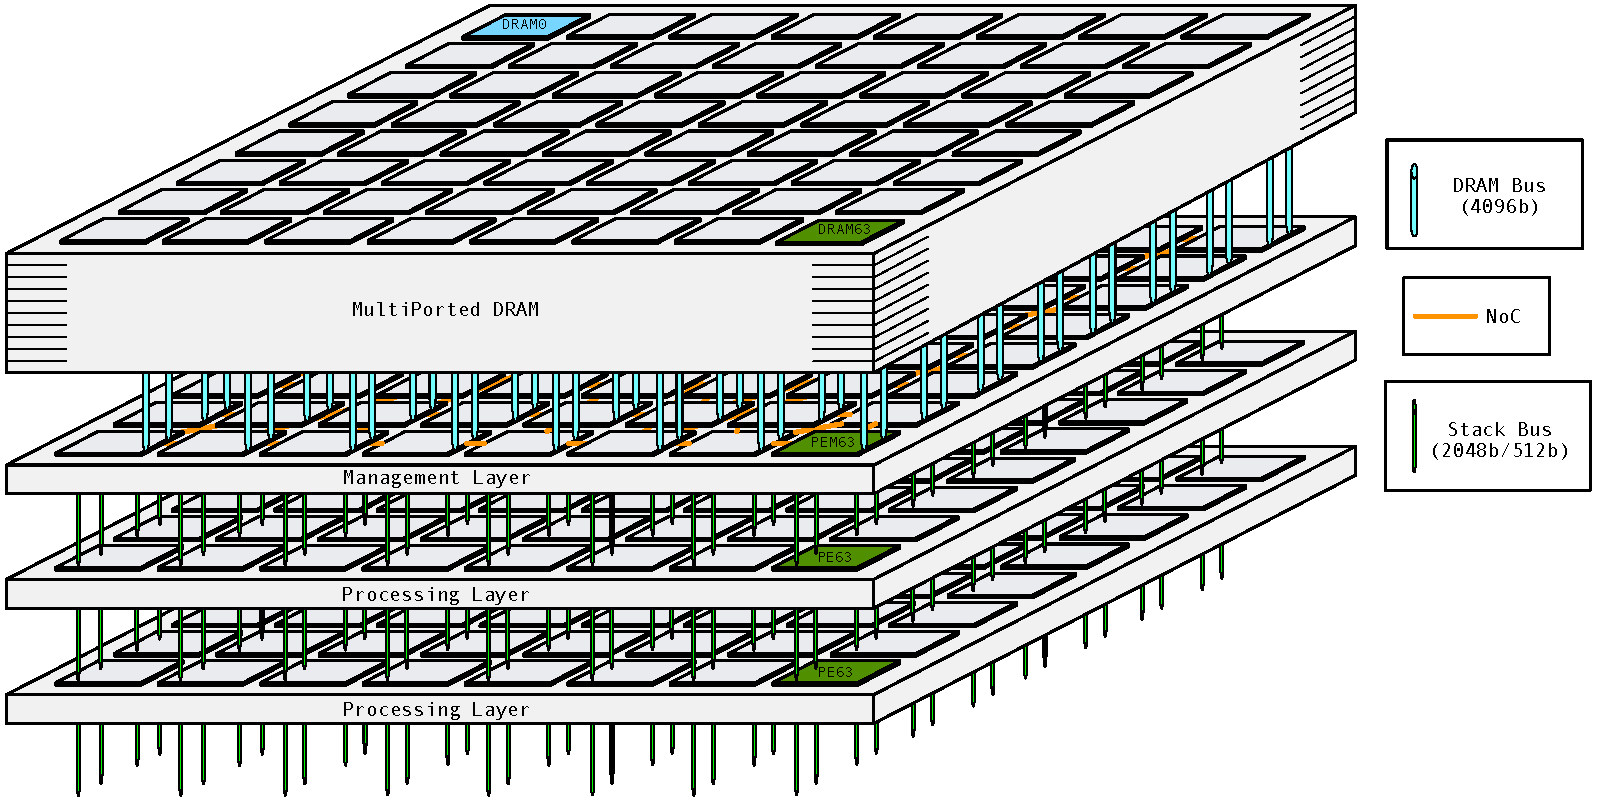
\includegraphics[width=.9\linewidth]{StackDiagram}}
}
\caption{3DIC System Stack}
\label{fig:3DICStack}
\end{figure}

3D-DRAM has recently become available in standards such as \ac{hbm} and \ac{hmc} and proprietary devices such as the DiRAM4 available from Tezzaron. 
These technologies provide high capacity within a small footprint.

In the case of \ac{hbm} and \ac{diram4} \cite{tezzaron:diram4}, the technology can be combined with additional custom layers to provide a system solution.

The question becomes, can a useful system coexist within the same 3D footprint?

This work targeted a baseline system with:
\begin{outline}
  \1 Computations requiring \ac{binary32}
  \1 Tezzaron \acf{diram4} \cite{tezzaron:diram4} for main memory
  \1 28nm \ac{asic} technology
\end{outline}
The work includes customizing the interface to a 3D-\ac{dram}, researching data structures to describe storage of \ac{ann} parameters, designing a memory manager with unique micro-coded instructions and a \ac{pe} layer.  
The targeted 3D-\ac{dram}, the Tezzaron DiRAM4 employs 64 disjoint memories arranged in a physical array.

This works system is designed such that a sub-system, known as a \acf{ssc} operates on one of the disjoint sub-memories within the \ac{diram4} (see figure \ref{fig:diram4Layout}).
As shown in figure \ref{fig:SSC}, the \ac{ssc} includes the \ac{diram4} sub-memory (referred to as the \ac{ssc} memory), a manager module and a \ac{pe} module.
The \ac{diram4} has 64 sub-memories so there are 64 \acp{ssc}. The \ac{ssc} has been designed as a standalone unit and does not have a knowledge of the other \acp{ssc} in the system.
\begin{figure}
\centering
\begin{subfigure}{.44\textwidth}
  \centering
  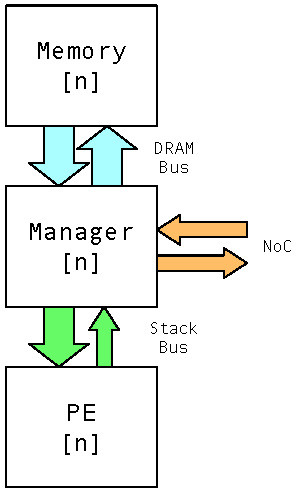
\includegraphics[scale=0.75]{SSC_logical}
  \captionsetup{justification=centering, skip=10pt}
  \vspace{-6pt}
  \caption{Sub-system column logical block diagram}
  \label{fig:Sub-system Column Logical Block Diagram}
\end{subfigure}%
\begin{subfigure}{.54\textwidth}
  \centering
  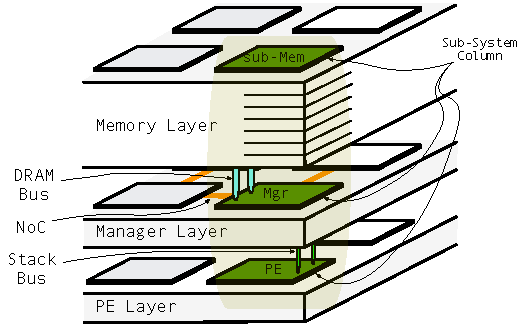
\includegraphics[scale=0.9]{SSC_physical}
  \captionsetup{justification=centering, skip=10pt}
  %\vspace{36pt}
  \vspace{20pt}
  \caption{Sub-system column physical diagram}
  \label{fig:Sub-system Column Physical Diagram}
\end{subfigure}
\captionsetup{justification=centering, skip=12pt}
\caption{\acf{ssc}}
\label{fig:SSC}
\end{figure}

An overview of the various blocks and interconnects are given in sections \ref{sec:3ddram} through \ref{sec:Overview Summary}
with additional detail provided in chapter \ref{sec:Detailed System Description}.

% ----------------------------------------------------------------------------------------------------
\section{Customized \ac{dram} : \acf{diram4}}
\label{sec:3ddram}
The \ac{diram4} \cite{tezzaron:diram4} employs multiple memory array layers in conjunction with a control and IO layer.
The memory is formed from 64 disjoint sub-memories each providing upwards of \SI[per-mode=symbol]{1}{\giga\bit} with a total capacity of at least \SI[per-mode=symbol]{64}{\giga\bit}.
Unlike traditional \ac{dram}, the \ac{diram4} has two independent channel which are accessed using \ac{ddr} signalling on the control signals.
Each channel has 32 banks and 4096 pages per bank with \SI[per-mode=symbol]{4096}{\bit\per page}.

The standard \ac{diram4} has a 32-bit read databus and a 32-bit write databus enabling simultaneous read and write. Both read and write databuses employ \ac{ddr} signaling.
The read and write transactions are burst-of-two providing 64bits per read/write. When accessing a \ac{dram}, a read and write are often referred to as a cacheline.
The device is designed to operate at \SI[per-mode=symbol]{1}{\giga\hertz} although this work targeted a \SI[per-mode=symbol]{500}{\mega\hertz} clock frequency.

This work is proposing customizations to the \ac{diram4} which are outlined in chapter \ref{sec:DRAM Customizations}. One of these proposed changes is to widen the read and write databuses to 2048-bits.
Using the same burst-of-two means each read and write will access an entire page. A cacheline becomes 4096-bits.
Another proposed change is the add mask bits to the write databuse to avoid having to perform read/modify/writes when writing back data much smaller than the new large cacheline.

\begin{figure}[!t]
% the [] contains position info e.g. [!t] means here
\centering
\captionsetup{justification=centering}
\captionsetup{width=.9\linewidth}
\centerline{
\mbox{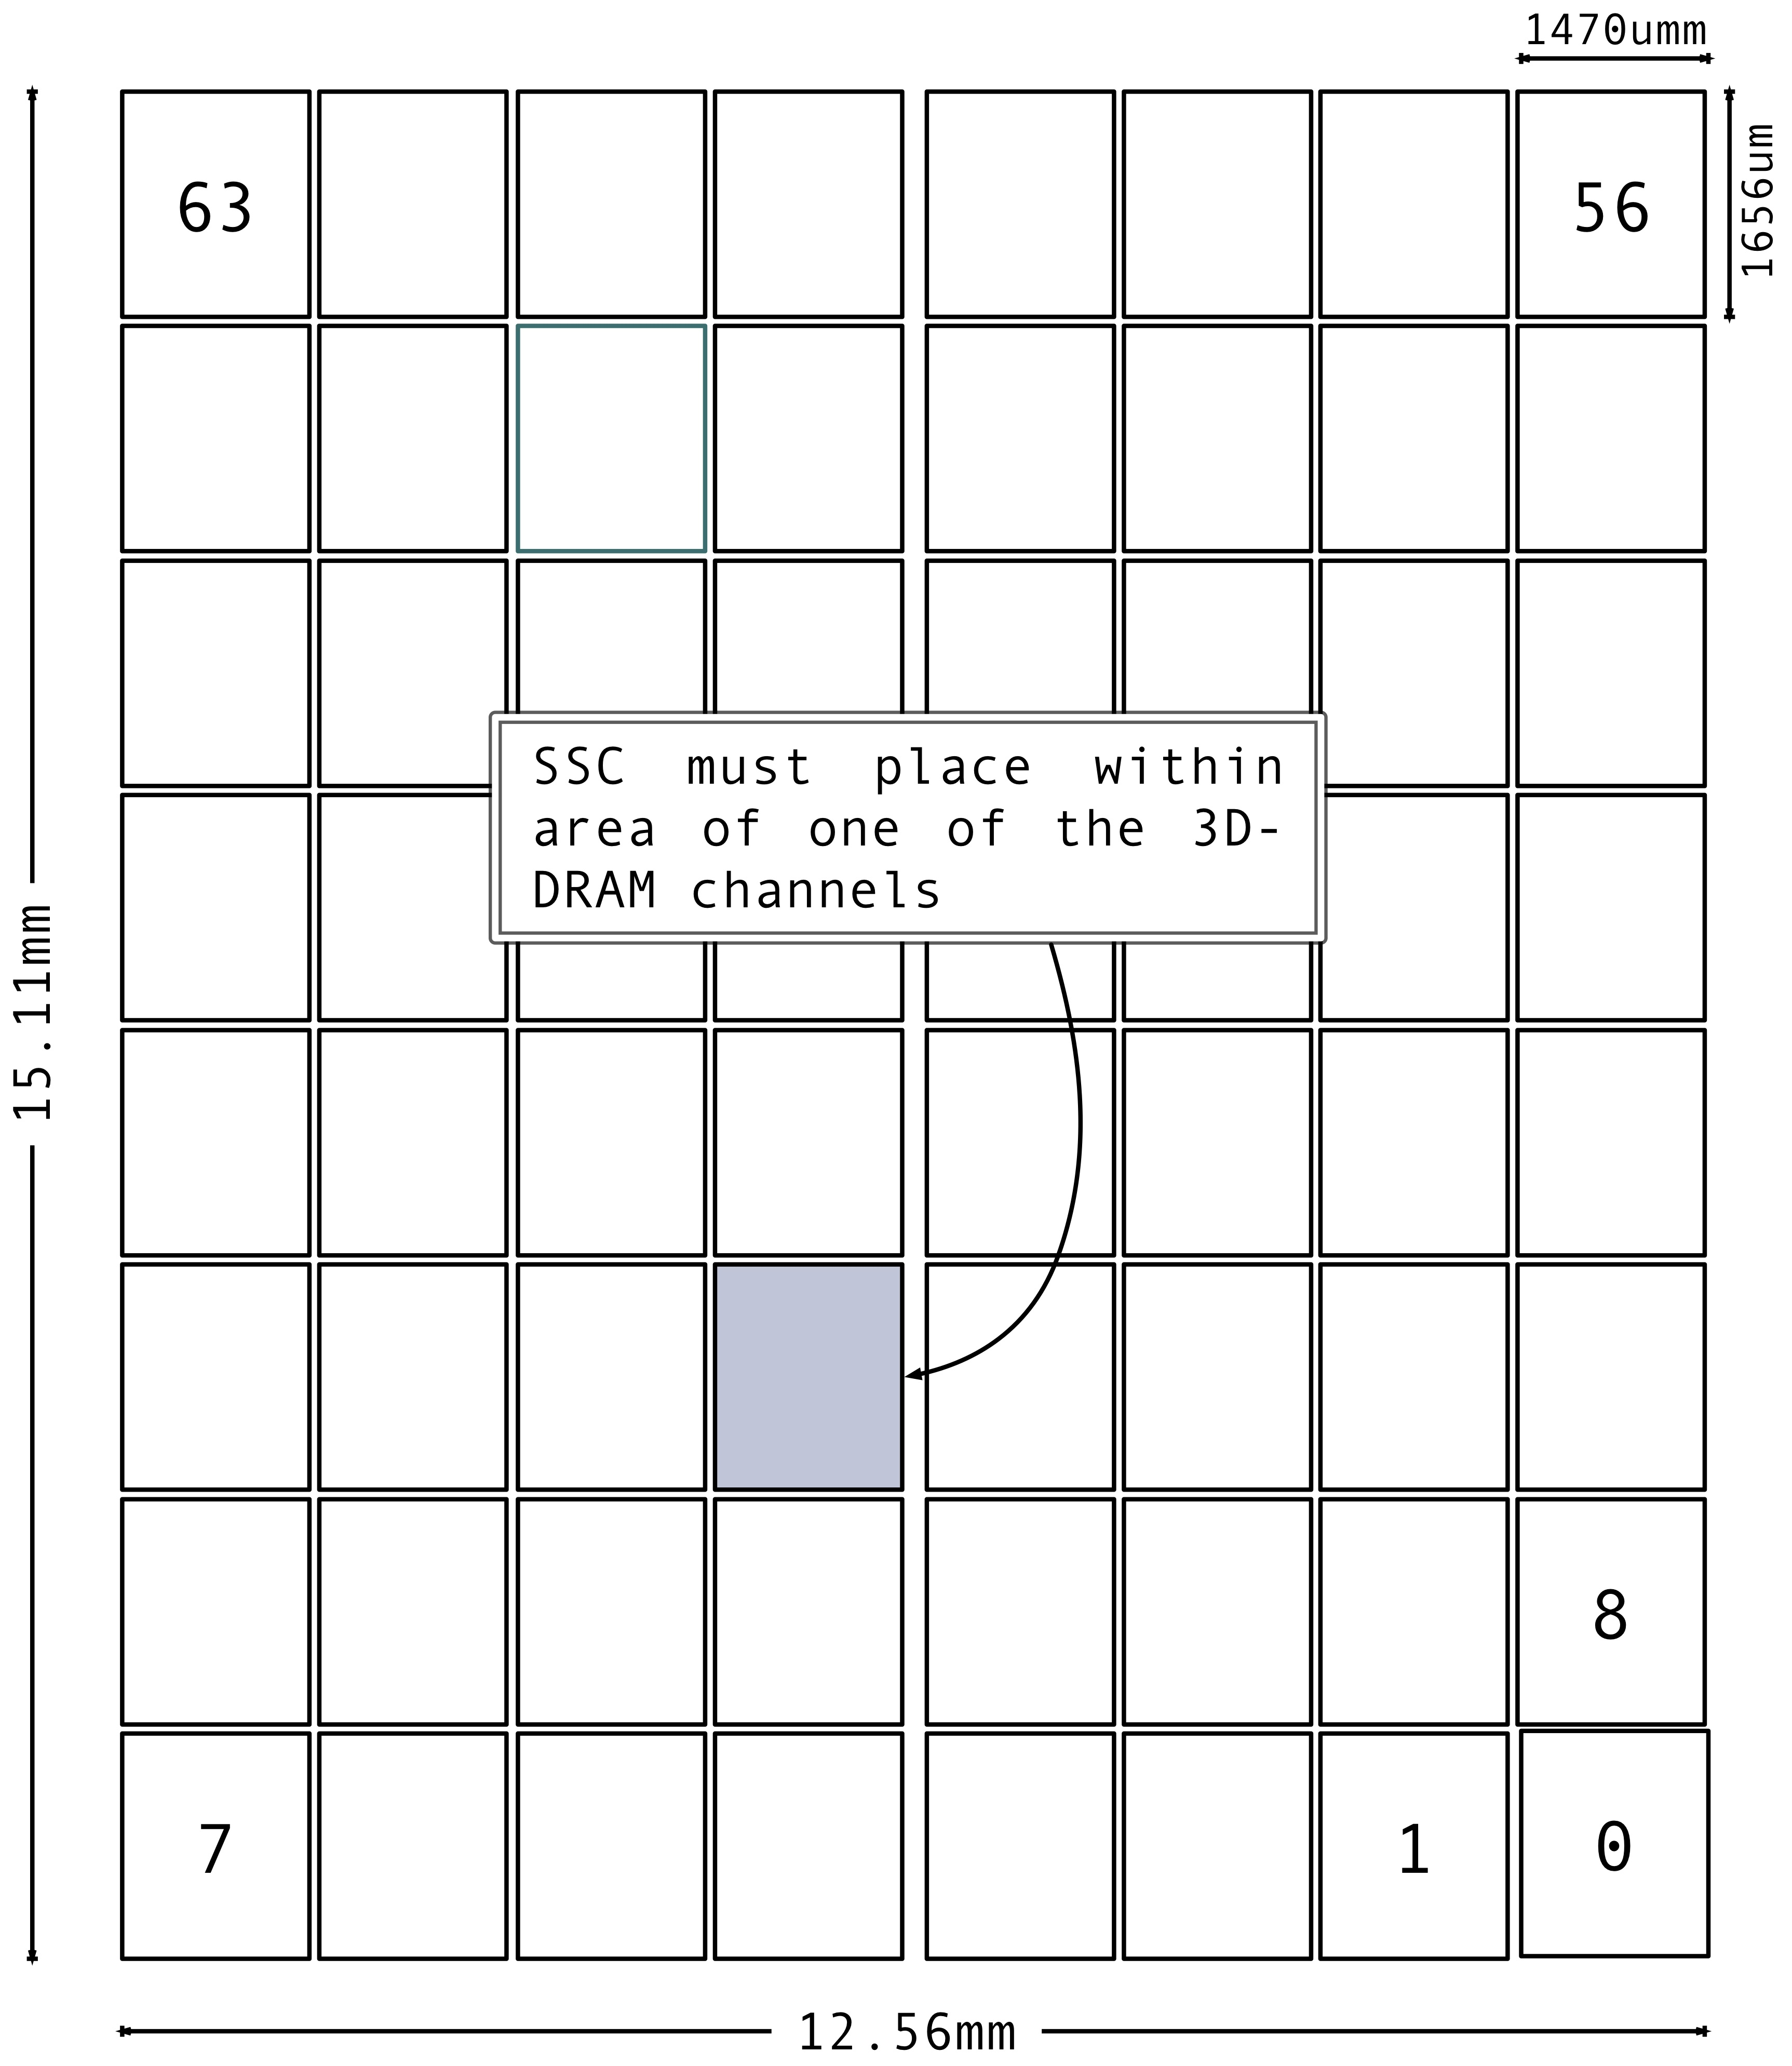
\includegraphics[width=.4\linewidth]{DiRAM4Layout}}
}
\caption{\ac{dram} Physical Interface Layout showing area for \ac{ssc}}
\label{fig:diram4Layout}
\end{figure}


% ----------------------------------------------------------------------------------------------------
\section{Layer Interconnect}
\label{sec:Layer Interconnect}

The layers are connected using through-silicon-vias (\ac{tsv}s) which provide high connection density, high bandwidth and low energy.
By ensuring the system stays within the 3D footprint ensures we can take advantage of the area and bandwidth benefits provided by \acp{tsv}.
The high density interconnect provided by \acp{tsv} allows the system to take advantage of the very wide \ac{dram} bus provided by the \ac{dram} customization described in section \ref{sec:Very-Wide Bus}.
The wide interconnect between the manager and \ac{pe} are also implemented using \acp{tsv}.

The interconnect between the manager and \ac{pe} is referred to as the stack bus. The interconnect between the manager and \ac{dram} is referred to as the \ac{dram} bus.

\subsection{Stack Bus}
\label{sec:Stack Bus}

The stack bus is bidirectional with a 36-bit \ac{oob} configuration bus from the manager to the \ac{pe}, a 2048-bit "downstream" data bus from the manager to the \ac{pe} and a 512-bit "upstream" data bus from the \ac{pe} to the manager.

The 36-bit \ac{oob} bus is designed to send configuration packets to configure the \ac{stop} and \ac{simd} blocks inside the \ac{pe}.
The packet primarily contains the \ac{stop} function to be performed on the downstream data and the operation the \ac{simd} is to perform on the result from the \ac{stop}.
It also includes the size of the downstream data stream and an operation idenfication tag.

The 2048-bit downstream stack bus is designed to carry 32 lanes of data with each lane containing two operand buses. 
In the baseline system, the two operand buses are designed to carry streams of \ac{binary32} numbers.
This allows the downstream stack bus simultaneously stream 32 execution lanes each with two 32-bit argument streams. 
Typically these streams are the weights and pre-synaptic \ac{an} states to calculate the states of up to 32 \acp{an}. 
The streams can also be configured to calculate the state of a single \ac{an} where the weights and pre-synaptic \ac{an} states for the single \ac{an} are sent in parallel across the downstream stack bus and a reduction operation can be performed in the \ac{pe} by the \ac{stop} and \ac{simd}.

The 512-bit upstream bus is primarily designed to send the results of a downstream operation. Typically this is the states of up to 32 \acp{an}.
The upstream bus is packetized with the result data contained in the data portion of the upstream packet.
Additional information includes the operation identification tag provided by the \ac{oob} command packet and the number of data words.
The upstream bus is not as wide as the downstream bus because the ratio of downstream operands to result data is a function of the pre-synaptic fanin.
Based on the average fanin from the baseline \ac{ann} shown in table \ref{tab:Layer Configuration}, a 512-bit bus exceeds the required average bandwidth.

The stack bus \ac{oob}, downstream and upstream signalling can be seen in figure \ref{fig:Stack Bus signalling}.

\subsubsection{Common Bus Signalling}
\label{sec:Common Bus Signalling}

With almost all interfaces in this system, additional control signals are used to a) validate, b) delineate and c) flow control messaging between blocks.
This "common" bus protocol signal group includes three signals, VALID, CNTL and READY. 
The single VALID signal is high when the bus contains valid information. The two bit CNTL signal is used to delineate by encoding \ac{som}, \ac{mom} and \ac{eom}.
Because of the asynchronous nature of the system, most interfaces employ small \acp{fifo}. When these \acp{fifo} are almost full, the source is flow controlled by the READY signal. 
The point at which the \ac{fifo} indicates the source to stop sending is based on the latency of the particular interface. 
The common signalling protocol will be seen in all waveform diagrams as seen in figure \ref{fig:Stack Bus signalling}.


\begin{figure}
\centering
\begin{subfigure}{.9\textwidth}
  \centering
  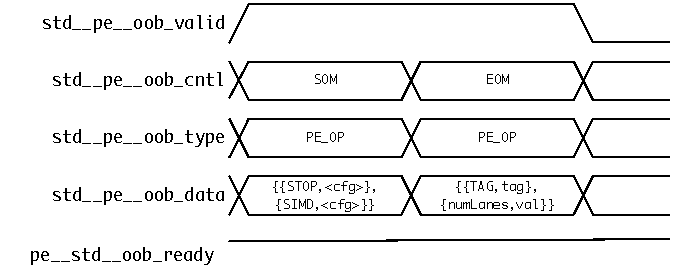
\includegraphics[width=0.7\textwidth]{stack_down_oob_wave_fig}
  \captionsetup{justification=centering, skip=10pt}
  \caption{Stack downstream OOB Bus}
  \label{fig:Stack downstream OOB Bus}
\end{subfigure}%

\bigskip

\begin{subfigure}{.9\textwidth}
  \centering
  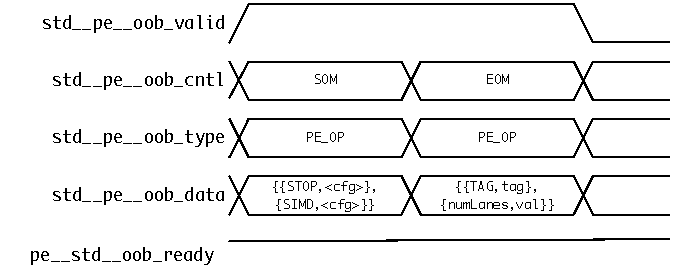
\includegraphics[width=0.7\textwidth]{stack_down_wave_fig}
  \captionsetup{justification=centering, skip=10pt}
  \caption{Stack downstream Data Bus}
  \label{fig:Stack downstream Data Bus}
\end{subfigure}%

\bigskip

\begin{subfigure}{.9\textwidth}
  \centering
  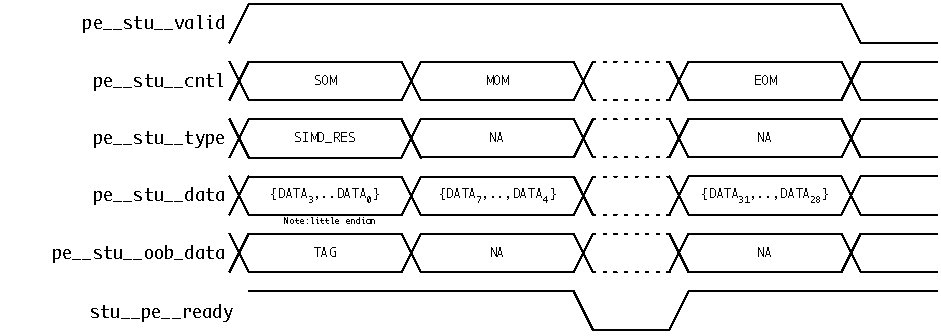
\includegraphics[width=0.7\textwidth]{stack_up_wave_fig}
  \captionsetup{justification=centering, skip=10pt}
  \caption{Stack upstream Bus}
  \label{fig:Stack upstream Bus}
\end{subfigure}%

\captionsetup{justification=centering, skip=16pt}
\caption{Stack Bus signalling}
\label{fig:Stack Bus signalling}
\end{figure}


\subsection{\ac{dram} Bus}
\label{sec:DRAM Bus}

The interface to the \ac{diram4} is similar to classic \ac{dram} interfaces with control signals including bank address and multiplexed page/cache address bus.
There are separate 2048-bit \ac{ddr} read and write databuses (see section \ref{sec:Very-Wide Bus}).
In total there are 4180 signals in the \ac{dram} interface.
Other than the wide databuses, the interface protocol is as described in \cite{tezzaron:diram4}.
A timing diagram showing a read and write to the \ac{diram4} are shown in figure \ref{fig:diram4Timing}.
\begin{figure}[!t]
\centering
\captionsetup{justification=centering}
\captionsetup{width=.9\linewidth}
\centerline{
\mbox{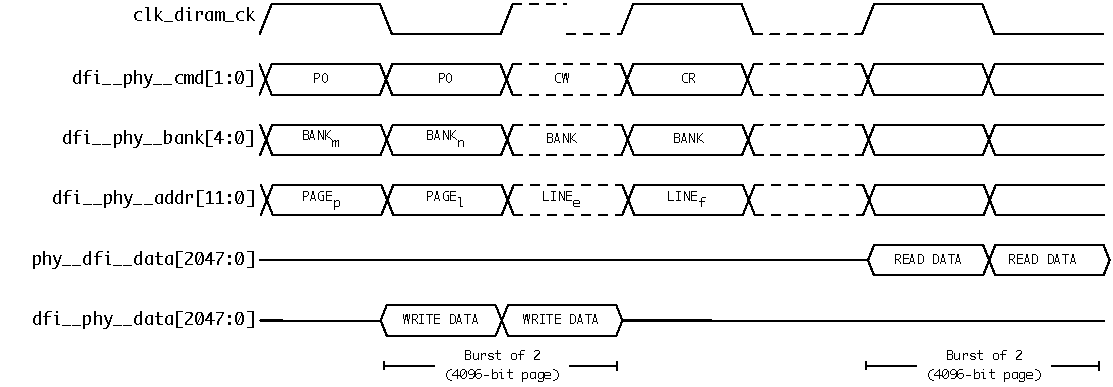
\includegraphics[width=.8\linewidth]{diram4TimingDiagram}}
}
\caption{Read and Write request to \ac{diram4} \cite{tezzaron:diram4}}
\label{fig:diram4Timing}
\end{figure}



The bandwidth of the \ac{dram} bus is designed to ensure data can be constantly maintained to the stack downstream bus.
Because an entire cacheline is accessed for each read request, there is an extreme case when back-to-back requests result in up to 32 \ac{dram} page opens commands.
It is possible that this sequence page opens could be followed by page closes resulting in a period when no useful data is being read from the \ac{diram4}.
This case is shown in figure \ref{fig:Worst case PO/PC sequence}.
\begin{figure}[!t]
\centering
\captionsetup{justification=centering}
\captionsetup{width=.9\linewidth}
\centerline{
\mbox{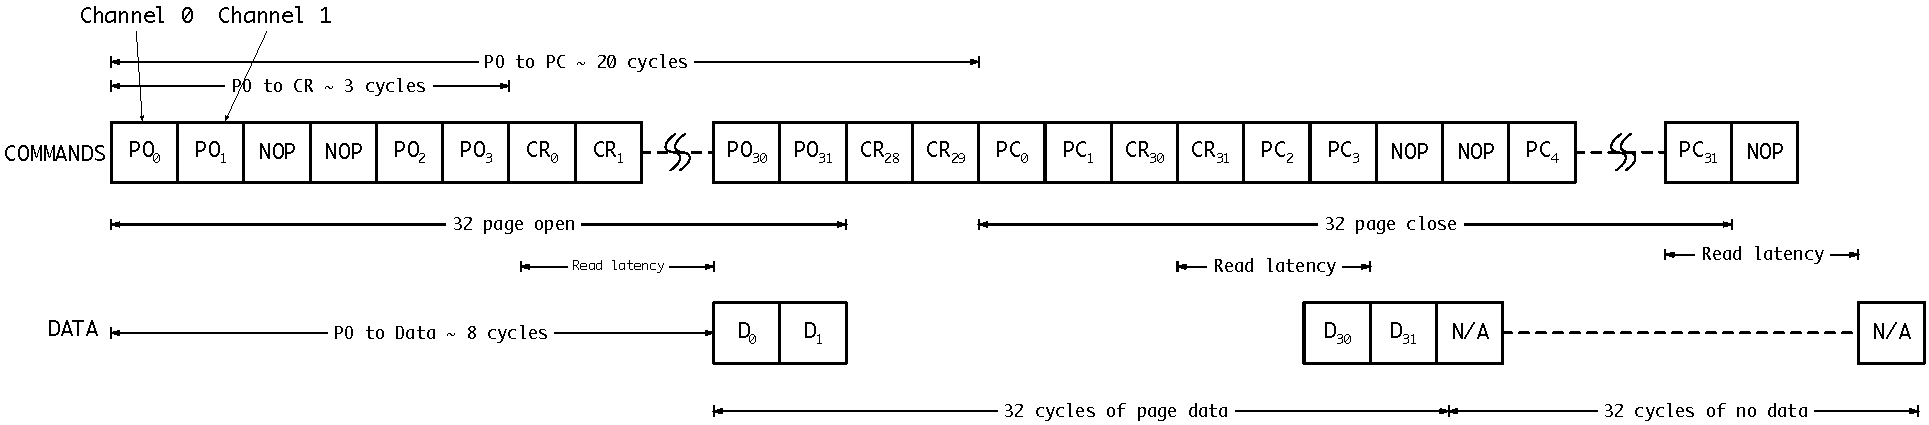
\includegraphics[width=1\linewidth]{worstCaseDiram4Read}}
}
\caption{Worst case PO/PC sequence}
\label{fig:Worst case PO/PC sequence}
\end{figure}
To accomodate this, the \ac{dram} bus has twice the raw bandwidth of the downstream stack bus. 
Therefore under this worst case scenario the higher bandwidth data from the \ac{diram4} must be buffered, as shown in figure \ref{fig:Worst case read path FIFO depth}.
In this case, per channel \SI[per-mode=symbol]{32}{\kilo\bit} \acp{fifo} must be placed in the read path as shown in figure \ref{fig:DRAM Read Path Buffering}.
These \acp{fifo} are instantiated in the managers memory read controller(s) as described in section \ref{sec:Memory Read Controller}.


\begin{figure}
\centering
\begin{subfigure}{.9\textwidth}
  \centering
  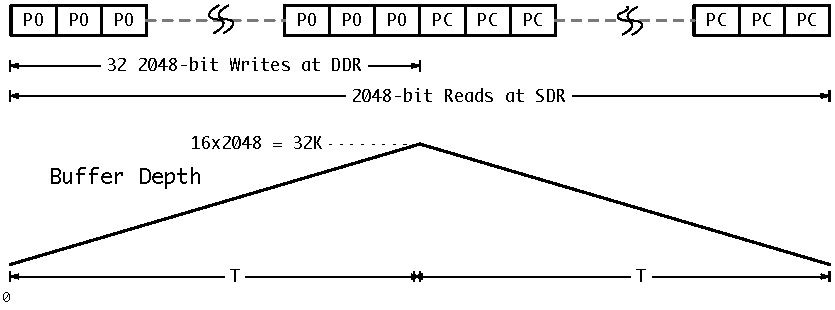
\includegraphics[width=0.7\textwidth]{readBufferDepth}
  \captionsetup{justification=centering, skip=0pt}
  \caption{Worst case read path FIFO depth}
  \label{fig:Worst case read path FIFO depth}
\end{subfigure}%

\bigskip

\vspace{-10pt}
\begin{subfigure}{.9\textwidth}
  \centering
  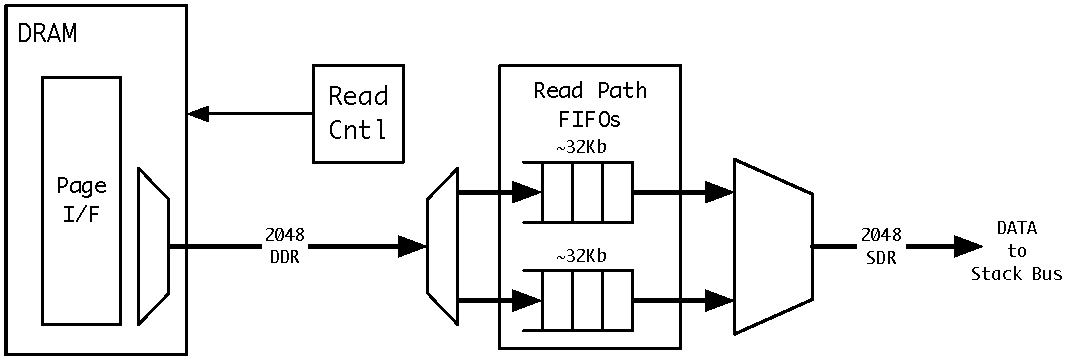
\includegraphics[width=0.75\textwidth]{readBufferBlockDiagram}
  \captionsetup{justification=centering, skip=6pt}
  \caption{Read path buffering diagram}
  \label{fig:Read path buffering diagram}
\end{subfigure}
\captionsetup{justification=centering, skip=16pt}
\caption{DRAM Read Path Buffering}
\label{fig:DRAM Read Path Buffering}
\end{figure}

\iffalse 
Each of the \ac{diram4} memories contain two channels with each channel containing 32 banks and each bank contains 4096 \SI[per-mode=symbol]{4}{\kilo\bit} pages.
\fi

% ----------------------------------------------------------------------------------------------------
\section{Manager Layer}
The Manager block is the main controller in the system. The operations required to process an \ac{ann} are formed from individual instructions which are decoded by the Manager. 
These instructions (for more detail see section \ref{sec:Instructions}) are sub-divided into descriptors to describe memory read operations, processing engine operations, memory write operations and general system operations for synchronization. 
The manager reads these system instructions from an instruction memory, decodes the descriptors and configures the various blocks in the system.
The configuration includes:
\begin{itemize}
      \item initiating operand reads from \ac{dram}
      \item preparing the processing engine (\ac{pe}) to operate on the downstream stack bus operand streams
      \item prepare the result processing engine to take the resulting \ac{an} activations from the \ac{pe} via the upstream stack bus and write those results back to the \ac{dram}
      \item replicate the resulting \ac{an} activations to neighbor managers over the \ac{noc} for processing of other \ac{ann} layers
\end{itemize}

The most common instruction is to perform \ac{an} state calculation on a group of \acp{an}.
This instruction contains four descriptors (see figure \ref{fig:Instruction 4-tuple}), an operation descriptor, two memory read descriptors and a memory write descriptor.
\begin{figure}[!t]
\centering
\captionsetup{justification=centering}
\captionsetup{width=.9\linewidth}
\centerline{
\mbox{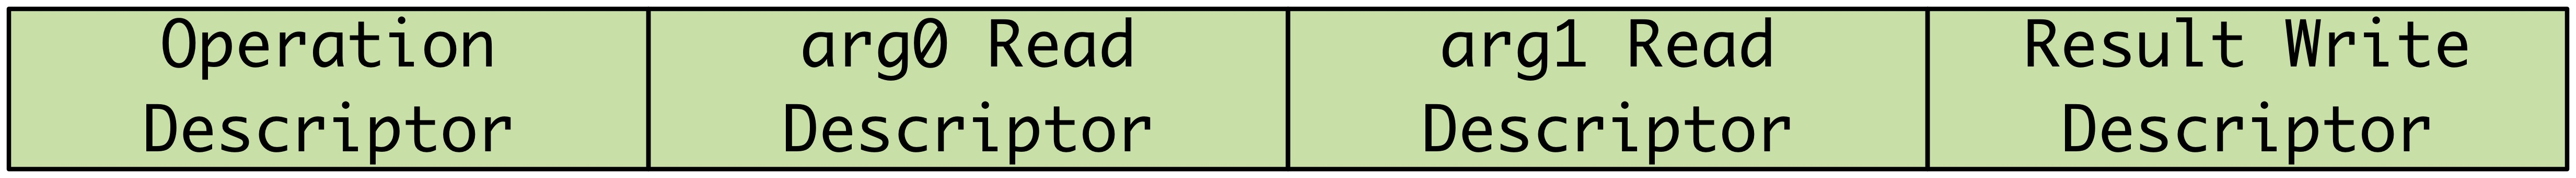
\includegraphics[width=.9\linewidth]{instruction4Tuple.jpg}}
}
\caption{Instruction 4-tuple}
\label{fig:Instruction 4-tuple}
\end{figure}


The operation descriptor describes the operations the \ac{pe} will perform, which typically includes a \ac{mac} to be performed by the \ac{stop} followed by a \ac{relu} function to be performed by the \ac{simd}.
The manager extracts the operation information, embeds the information in an \ac{oob} packet and sends the packet to the \ac{pe} over the downstream \ac{oob} bus.
The two memort read descriptors are used to define the memory locations of the downstream stack data buses. 
There is one memory read descriptor for each of the two operand streams in the execution lanes, one typically defines where the pre-synaptic weights are stored and one for where the pre-synaptic \ac{an} states are stored.
The architecture is designed to for an instruction to compute the state of multiple \acp{an} or for an individual \acp{an} state to be computed.
If a group of \acp{an} are computed, the pre-synaptic connection weights for the \acp{an} are stored interleaved and when read from \ac{dram} are directed to one of the streams of each of the execution lanes.
If a single \ac{an} is computed, the pre-synaptic connection weights for the \acp{an} are stored linearly and when read from \ac{dram} are directed to one of the streams of each of the execution lanes.
The pre-synaptic \ac{an} states are stored in row-major order and when read are broadcast to the other stream of each execution lane.



% ----------------------------------------------------------------------------------------------------
\section{Processing Engine Layer}
\label{sec:Processing Engine Layer}
The \ac{pe} contains two main processing modules, the \ac{stop} and the \ac{simd} block.
Both the \ac{stop} block and the \ac{simd} have 32 execution lanes. The execution lanes inside the \ac{stop} contain functions required to perform \ac{an} related operations.
The \ac{simd} will be based on the device described in \cite{schabel2014diss}.


The \ac{pe} is configured by the manager to perform operations on two operand data streams from the manager. 
The \ac{stop} is able to operate on this data directly from the manager at the full bandwidth rate of the stack bus and does not have to be stored in local \ac{sram} prior to processing. 
There is a small \ac{fifo} to provide buffering to allow asynchronous configuration of the \ac{stop} block and the source of the streaming data in the manager. 
The \ac{fifo} also allows the two argument streams in each of the execution lanes to wander with respect to each other and with respect to the other lanes.

The architecture is expandable to allow various functions to be provided in the \ac{stop}.
The current baseline implementation includes the \ac{mac} operation.
There is a \acp{mac} per execution lane allowing up to 32 simultaneous pre-synaptic \ac{an} $weight \cdot state$ computations on the two operands from the two streams in each execution lane.
These computations can be for a group of up to 32 \acp{an} or for a single \ac{an} as shown in figure \ref{fig:PE AN calculation}.

\begin{figure}
\centering
  \begin{subfigure}{.49\textwidth}
    \centering
    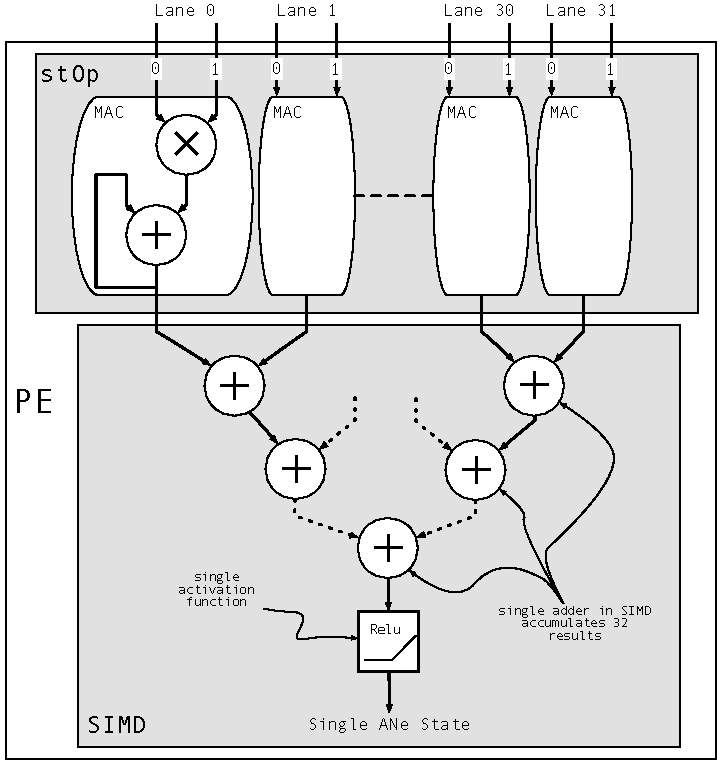
\includegraphics[width=0.9\textwidth]{singleANcalculation}
    \captionsetup{justification=centering, skip=10pt}
    \caption{Single ANe calculation}
    \label{fig:Single AN calculation}
  \end{subfigure}%
%\bigskip
  \begin{subfigure}{.49\textwidth}
    \centering
    \vspace{40pt}
    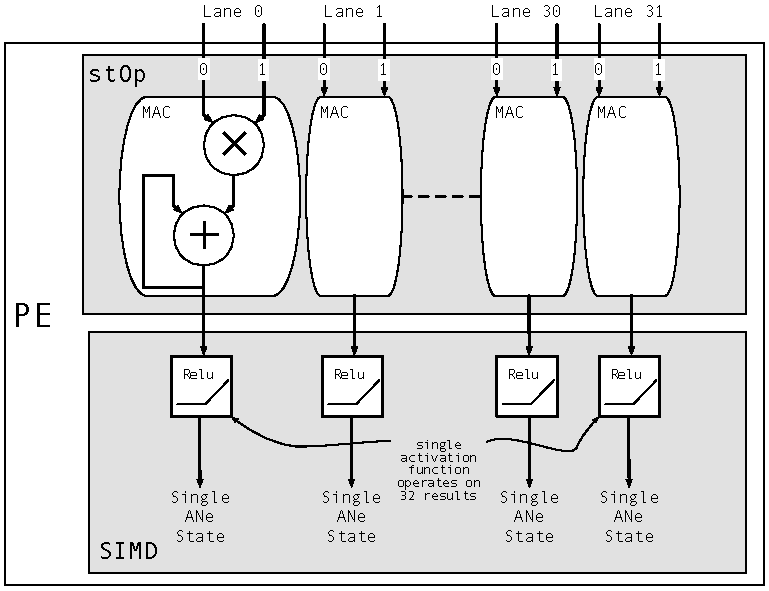
\includegraphics[width=0.9\textwidth]{groupANcalculation}
    \captionsetup{justification=centering, skip=10pt}
    \caption{Group ANe calculation}
    \label{fig:Group AN calculation}
  \end{subfigure}%
\vspace{-10pt}
\captionsetup{justification=centering, skip=16pt}
\caption{\ac{pe} \ac{an} calculation}
\label{fig:PE AN calculation}
\end{figure}

If it is for a group of \acp{an}, the \ac{simd} only has to perform the activation function on the 32 results from the \ac{stop}. 
If a single \ac{an} is being processed, the \ac{simd} must accumulate the result from each execution lanes \ac{stop} before applying the activation function.
The activation function currently implemented is the \ac{relu}.
The \ac{an} states can be sent back to the manager over the stack upstream bus or retained for further processing such as pooling or softmax calculations.

% ----------------------------------------------------------------------------------------------------
\section{Inter-Manager Communication}
\label{sec:Inter-Manager Communication}

During configuration and/or computations, it may be required to replicate data to other \acp{ssc}.
During \ac{an} computations, an \ac{ssc} only reads \ac{ann} weights and states from its local \ac{dram} and not \ac{dram} of other \acp{ssc}.
In some cases, such as fully connected layers and locally-connected layers with \ac{roi} overlap, the \ac{an} computation in an \ac{ssc} for layer $n$ may include \ac{an} states from layer $n-1$ which were computed in another \ac{ssc}.
In this case, when \acp{an} are being computed for layer $n-1$, the operation instruction contains information as to where the result should be written back for computing \acp{an} in layer $n$.
If a particular layer $n-1$ \ac{an} is required by another \ac{ssc} when computing a layer $n$ \ac{an}, the result is sent to all dependent \ac{ssc} via the \ac{noc}.
The instruction contains one or more storage descriptors (see section \ref{sec:Storage Descriptor}) that identify the destination of the operation result.
If the result must be replicated, there are multiple storage descriptors. When the result is returned by the \ac{pe}, the manager examines the storage descriptors and determines which \ac{ssc} the result should be sent.
The manager creates an \ac{noc} header which includes information on all the destination \acp{ssc}. 
This is encoded as a 64-bit field although the \ac{noc} header supports a multicast group. 
The multiple storage descriptors and the result data are placved in the data portion of the \ac{noc} packet.
As the packet traverses the \ac{noc}, it is replicated to outgoing ports based on the destination bit field.
When the destination \ac{ssc} receives the packet, it extracts the storage descriptor and writes the data to its local \ac{dram}.
The \ac{noc} packet format can be seen in figure \ref{fig:NoC packet format}.
This inter-manager communication is provided by an \ac{noc} with all managers connected in a mesh as shown in figure \ref{fig:Mesh}.
\begin{figure}[!t]
% the [] contains position info e.g. [!t] means here
\centering
\captionsetup{justification=centering}
\centerline{
\mbox{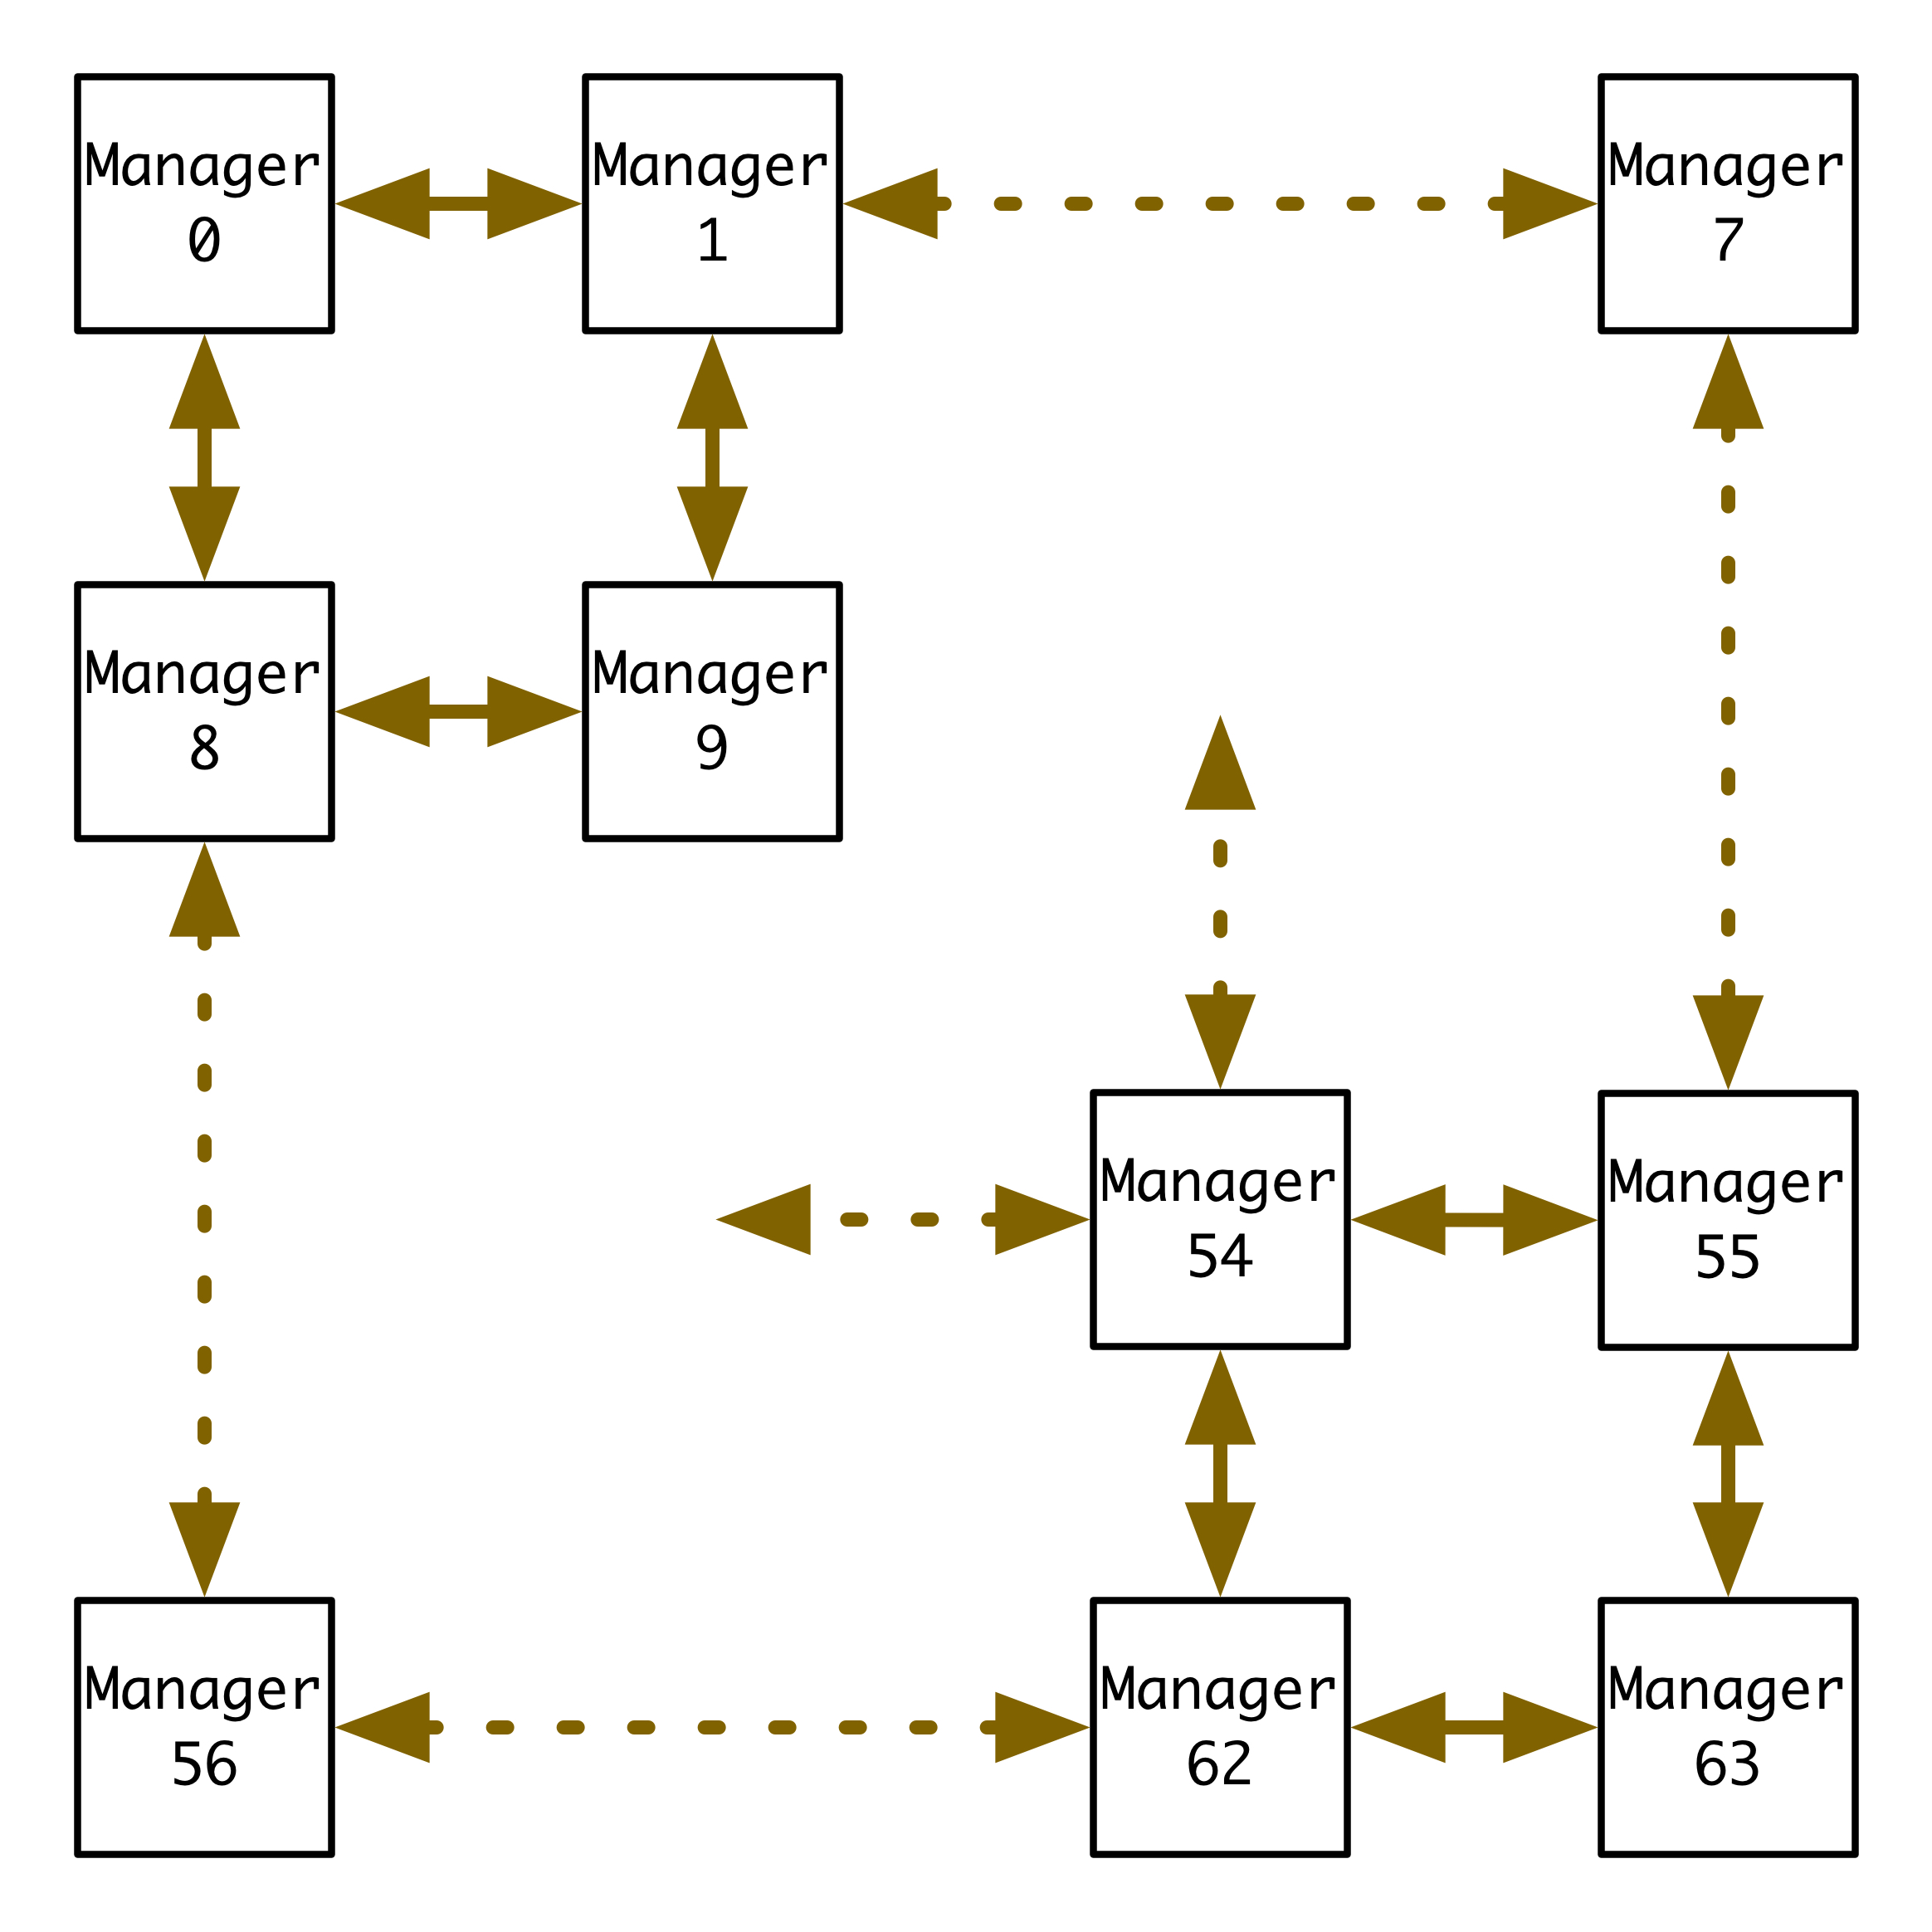
\includegraphics[width=.5\linewidth]{Mesh}}
}
\caption{\ac{noc} manager connectivity}
\label{fig:Mesh}
\end{figure}

\begin{figure}[!t]
\centering
\captionsetup{justification=centering}
\captionsetup{width=.9\linewidth}
\centerline{
\mbox{\includegraphics[width=.9\linewidth]{nocpacket}}
}
\vspace{-10pt}
\caption{\ac{noc} packet format}
\label{fig:NoC packet format}
\end{figure}


When computing an \ac{ann} across multiple processing sub-systems, often \ac{an} activation data must be shared between these \ac{ssc}s. The \ac{ssc} includes the \ac{dram} port, the manager and the \ac{pe}. 
An \ac{noc} within each management block communicates with each adjacent manager using a mesh network. This \ac{noc} has a forwarding table that can be reconfigured to provide more efficient routing for a given processing step.

Each manager has an integrated \ac{noc} module that has four ports. 
The managers in the middle of the array use all four ports to connect to adjacent managers.
The managers in the corners of the array connect to two adjacent managers.
The managers at the edges connect to three adjacent managers.
The host is connected to one (or more) of the managers at one edge of the array. 

% ----------------------------------------------------------------------------------------------------
\section{Summary}
\label{sec:Overview Summary}

A control and data flow diagram of the stack showing the 64 sub-system columns can be seen in figure \ref{fig:FlowDiagram}.
\begin{figure}[!t]
% the [] contains position info e.g. [!t] means here
\centering
\captionsetup{justification=centering}
\centerline{
\mbox{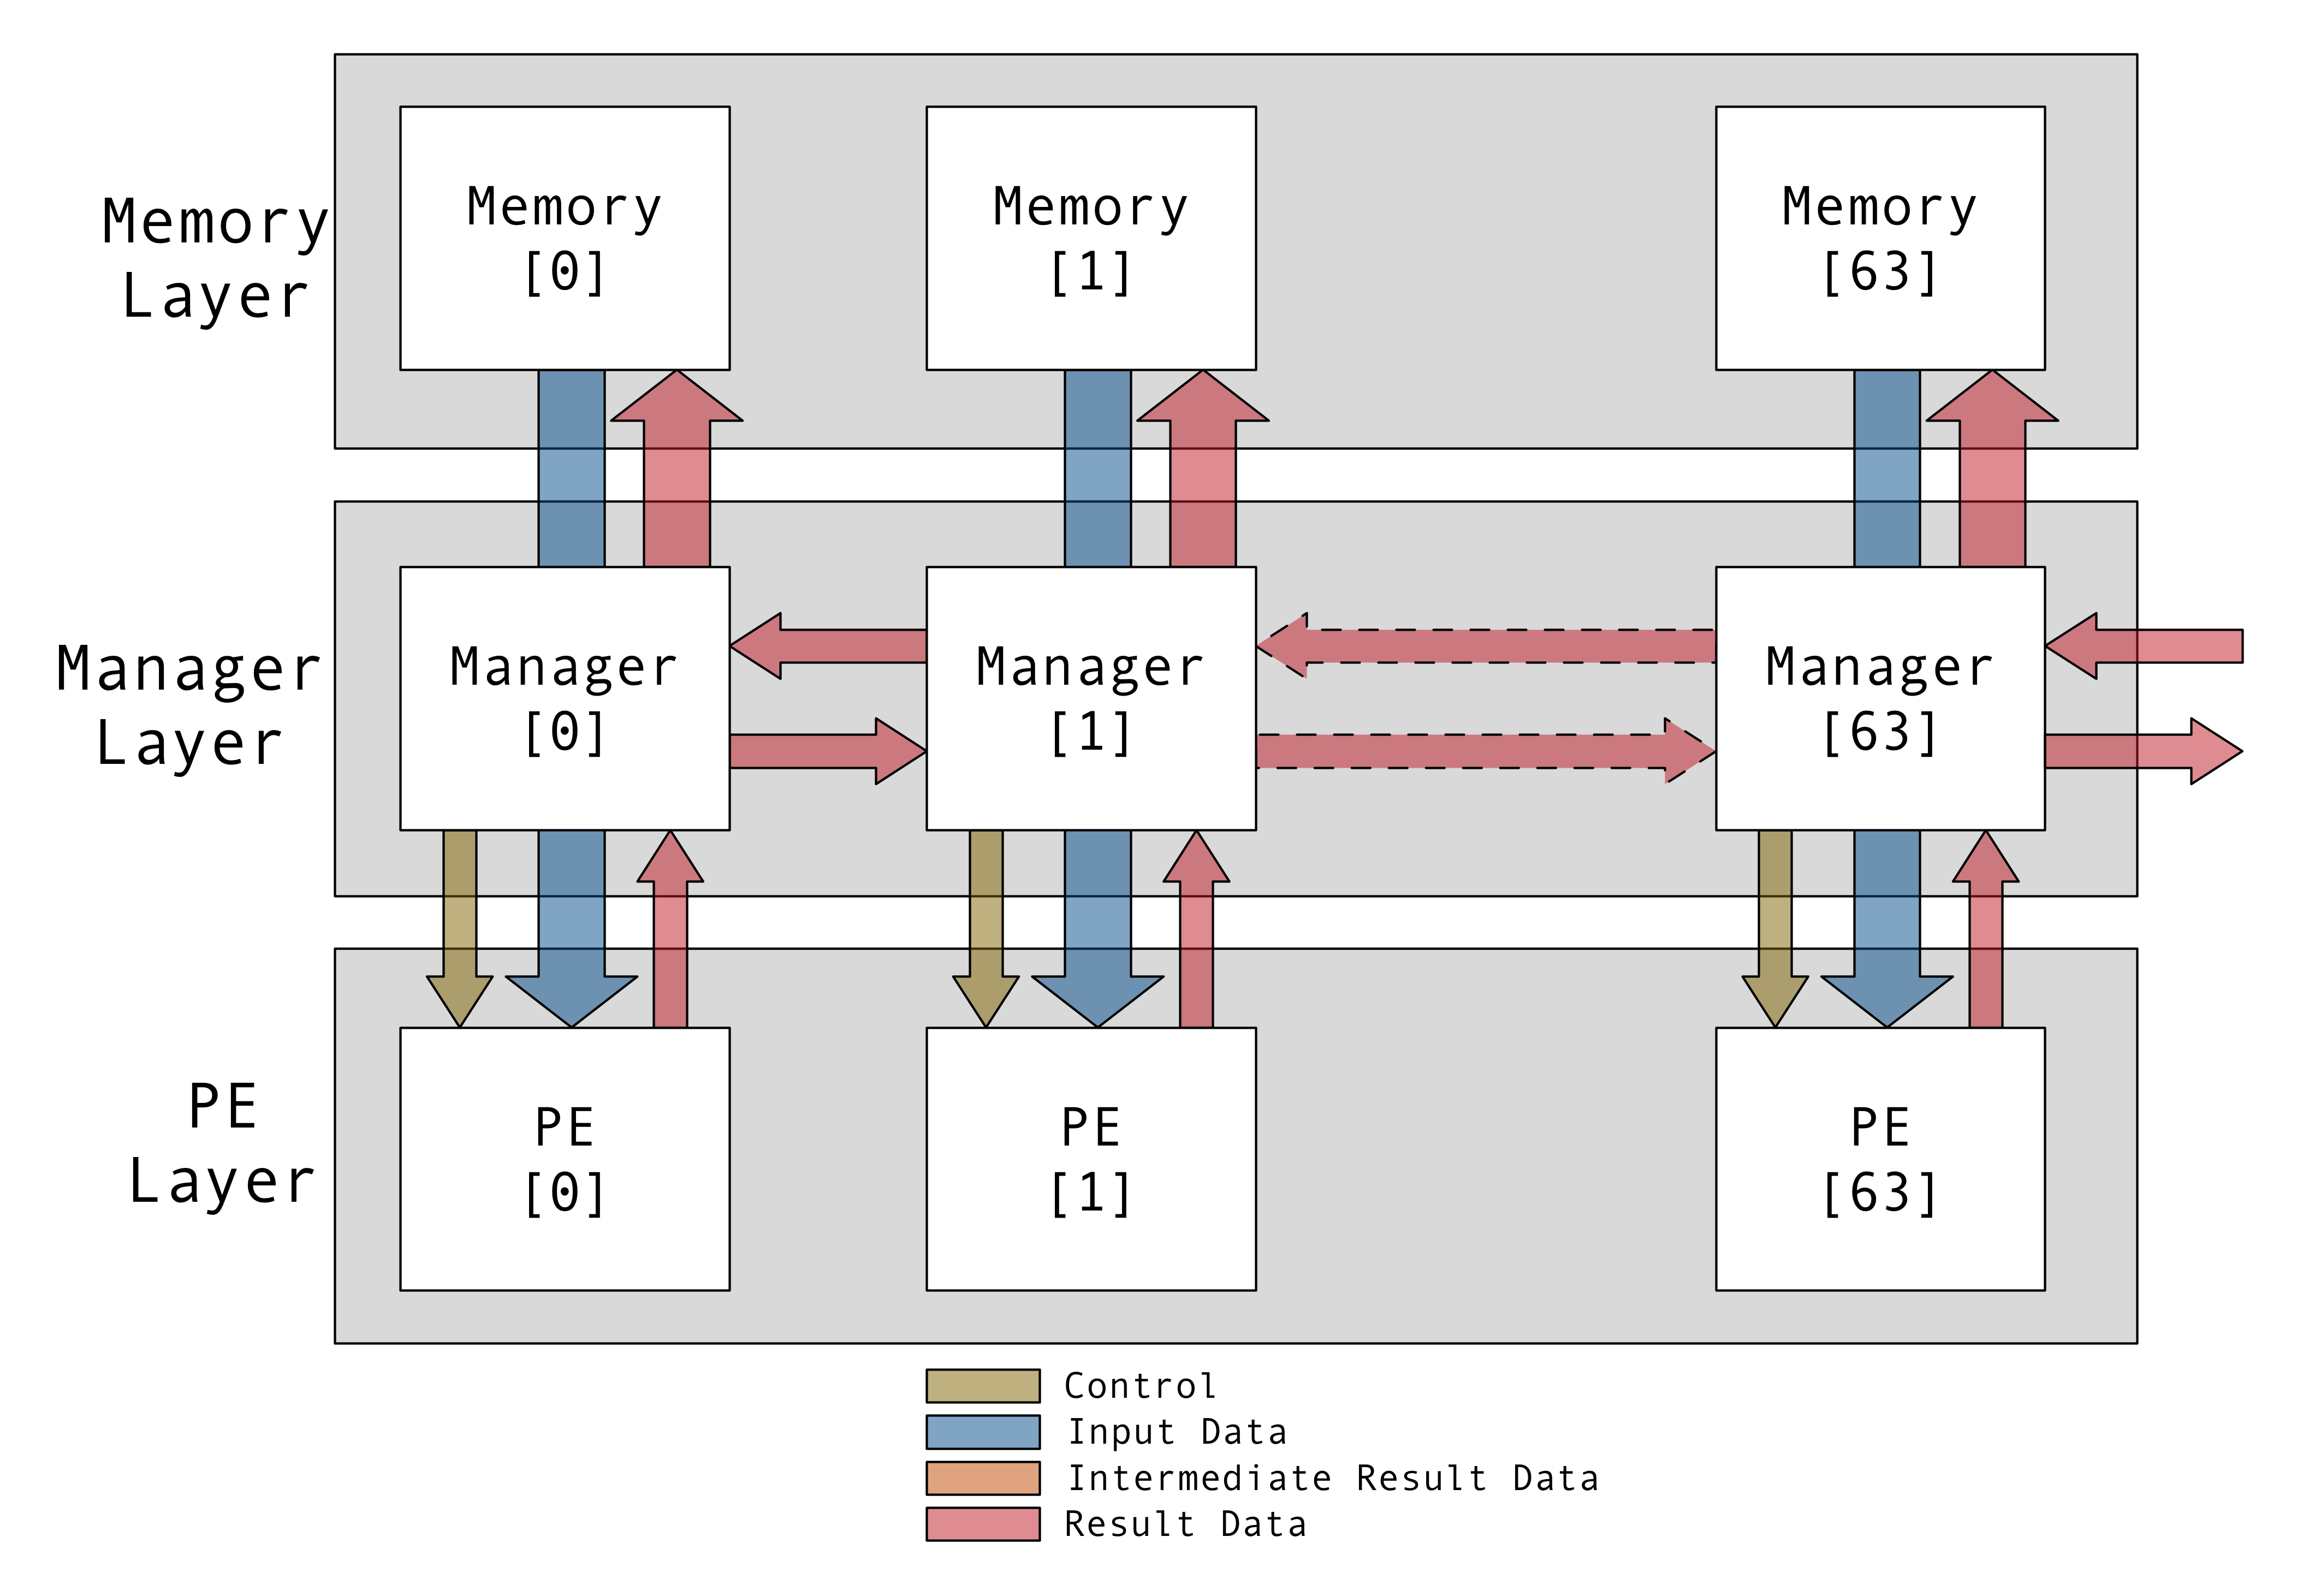
\includegraphics[width=.8\linewidth]{FlowDiagram.jpg}}
}
\caption{System Flow Diagram}
\label{fig:FlowDiagram}
\end{figure}

\subsection{Configuration, Command and Data Flow}
\label{sec:Configuration, Command and Data Flow}


**** WIP ****

The host is responsible for loading each managers instruction memory over the \ac{noc} and a main controller module in the manager.
The host sends a command to start the manager decoding a defined number of instructions at a specific address in the instruction memory.

The manager decodes instructions and sends control commands to various modules in the manager and the \ac{pe}.

One module, the \ac{oob} downstream channel sends configuration packets to the \ac{pe} over an \ac{oob} channel embedded in the stack bus.
This configuration packet includes a) a pointer to a pre-programmed operation to be performed by the streaming operation module on the data streams to the \ac{pe} and b) a pointer to a pre-programmed portion of the \ac{simd} instruction memory which defines the operations to be performed by the \ac{simd} on the result of the streaming operation block.
 in the \ac{pe}commwhich is a part of the is instructed to send \ac{simd} and \ac{stop} commands over an out-of-band channel in the stack bus to the \ac{pe}.
The managers at the edge of the array The host is connected to one (or more) of the managers at one edge of the array. EachAll communication between \acp{ssc} is over an \ac{noc}. 
Some causes of communication between \acp{ssc} are host configuration, synchronization messages between \acp{ssc}, \ac{an} state replication etc..
\iffalse
Synchronization messages and \ac{an} state replication are a side effect of the instructions described in chapter \ref{sec:SystemOperations}.
\fi


